\chapter{研究现状和相关工作}
本章介绍研究现状和相关工作。

\section{视频流媒体领域的研究现状}

视频流媒体的研究可以从系统模块的角度分为几个方面。一是数据源端,即视频编码的研究,如何提高压缩率,如何提高码流的可伸缩性。二是传输过程,如何改善网络状况,如何充分合理利用带宽资源。三是客户终端,如何快速解码和更好的显示。

\section{SVC码流截取的相关工作}

\subsection{问题描述}

码流截取是从一个完整的SVC码流中抽取所有数据包的一个子集,得到一个更低码率的子流的过程。图\ref{fig:Bitstream-Extraction}展示了一个SVC码流的结构,以及从中截取子流的一种可能的方式。
可以看到,该码流中的数据包被分为了不同的层。时间层(T0~T3)反映了各帧之间的参考或依赖关系。图形上方的箭头从被参考帧指向参考它(也就是依赖于它)的帧。质量层(Q0~Q2)反映了一帧之内的视频质量伸缩性。处于高层(也就是Q1和Q2层)的数据包可以被部分丢弃从而实现码流截取。图中的虚线表示了一个截取的例子。虚线上方的数据包全部被丢弃,只有虚线下方的数据包保留在截取出来的子流中。

\begin{figure}[h]
\centering
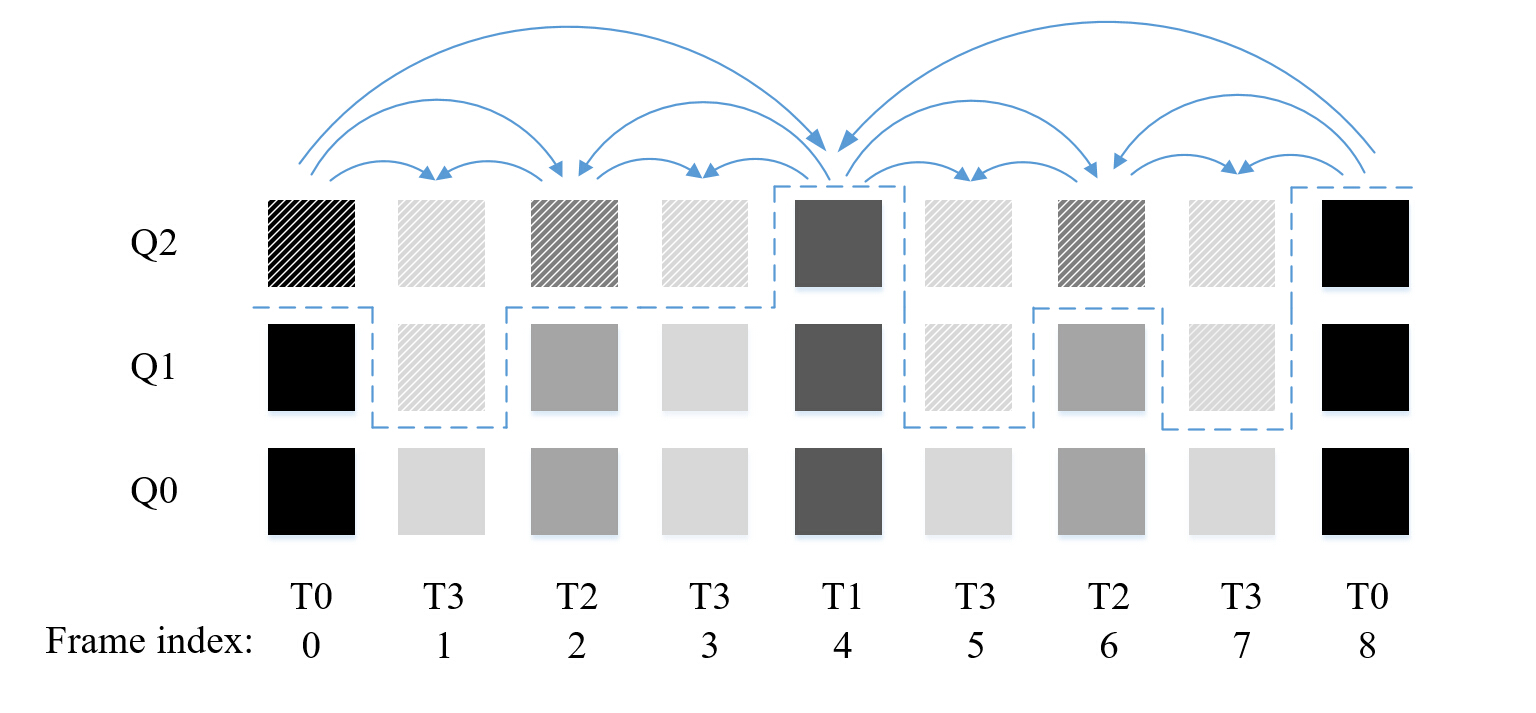
\includegraphics[width = 0.9\linewidth]{./figures/Bitstream-Extraction.jpg}
\caption{可伸缩视频码流截取 \label{fig:Bitstream-Extraction}}
\end{figure}

容易发现,SVC码流截取从本质上来看其实是一个组合优化问题。在所有的数据包中,我们希望在给定的码率限制下,选出一个最优的数据包组合,使得它们构成的子流具有最大的视频质量。更准确地说,这个问题与大家所熟知的“0-1背包问题”\footnote{http://en.wikipedia.org/wiki/Knapsack\_problem}在形式上是一致的。每个数据包可以看作是一个具有特定重量和价值的物品。这里的重量就是数据包的大小,价值就是它对重建视频质量的贡献。码流截取的过程就是决定每个数据包是否包含在最终的子流里。用“0-1背包问题”中的术语来说,就是选择将哪些物品放入背包中。

对于典型的“0-1背包问题”而言,其最优解可以用动态规划的方法得到。然而对于码流截取问题来说,这个方法是不可行的。主要原因在于数据包之间的依赖关系。首先,截取的数据包子集不能任意挑选,因为如果一个包被包含进了子流中,那么这个包所依赖的数据包也必须被包含进去,否则将无法正确解码。例如,在图\ref{fig:Bitstream-Extraction}中,我们不能只选择一帧中的Q2层数据包而丢弃同一帧的Q1层。其次,不同于“0-1背包问题”中定义良好的物品价值,码流截取问题中一个数据包对最终视频质量的贡献并不是明显且确定的。这是因为,数据包所在的帧在解码中是互相参考的,它们对视频质量的影响会互相干扰,对于不同的截取方案,每个数据包的实际贡献可能有所不同。事实上,除非实际进行一遍截取、解码、计算的操作,我们甚至无法准确地得到所截取出的子流的真实视频质量。这就使得SVC码流截取问题成为了一个复杂得多的问题。

\subsection{相关工作简介}

就我们所知,学术界没有人提出过一种确定能找到码流截取最优解的方法。当然可以用暴力穷举的方法来解决这个问题,但其复杂度显然是无法接受的。相关的工作都是尽可能用较低的计算获得较好的次优解。下面对SVC码流截取的相关工作做简要的介绍。

Amonou等人\supercite{Amonou2007}提出了一个基于“Quality Layers”的码流截取方案。这一方案被SVC参考软件JSVM\supercite{JSVM}所采用,而且取得了比JSVM中的基本截取器更好的性能。在Amonou等人的方案中计算了一个“Quality Layers”(简称QL)值,它反映了一个数据包的码率失真影响,据此进行截取能得到率失真优化过的结果。但估计一个数据包的失真影响是一个计算量非常大的过程,而且失真估计的准确性也有提高的空间。因此,后续的工作提出的失真模型一方面是降低复杂度,另一方面是进一步提高准确度。Sun等人\supercite{Sun2009}和Maani等人\supercite{Maani2009}所构造的模型都是基于帧间的误差漂移来计算失真。孙等人的模型在性能方面几乎与JSVM相当,但计算复杂度却大大减少。而Maani等人的模型取得了比JSVM更高的估计准确度,但是由于其是基于训练的,为了得到更鲁棒的模型参数,需要更大的计算量。

Ramanathan等人\supercite{Ramanathan2012}提出了一个“Quality Metadata”的概念来用于码流截取,这与上面所说的“Quality Layers”是同样的思想,只是计算方法有所差别。Yang等人\supercite{Yang2013}提出了一个基于模拟退火的方法来解决码流截取问题。因为码流截取从另一个角度看是丢弃数据包的过程,丢弃的先后顺序可以认为是这些数据包的优先级。于是一些研究者从赋优先级的角度来提出相应的算法。例如,Lim等人\supercite{Lim2006}把SVC码流视为树形结构并据此来为每个数据包赋予优先级,而Zhu等人\supercite{Zhu2011}则采用拉格朗日乘子方法计算优先级值。在这些已有的工作中,失真估计的准确性都显著地影响最终结果。因此,提出简单有效的误差或失真模型对于码流截取的研究至关重要。这正是本文的创新点之一。


\section{码率自适应的相关工作}

\subsection{问题描述}

在数据源具备码率可变的前提条件之后,实际传输时就可以根据带宽来调整发送的速率。改变码率去适应带宽的变化,这就是所谓的码率自适应问题。对于一个码率自适应算法,有三个最基本的目标。这三个目标可以用来衡量自适应算法的效果,也是设计算法时需要考虑的方面。下面分别进行描述。

首先是要确保视频播放的连续性。在流媒体系统中,一旦视频开始播放,每个数据包都有了自己的显示时间。这个时间也决定了传输的截止时间。如果这个数据包没有在截止时间前达到客户端,那么客户端播放器就会因缺少数据而暂停。这就是用户所遇到的卡顿现象,应该努力避免。

第二个目标是保持视频质量的平滑性。网络条件变化可能比较剧烈,但视频质量应该尽可能维持在一个比较稳定的水平。因为频繁的质量调整会给用户带来反感。举例来说,当用户适应了较低的质量后,突然调高质量并在短时间内又调低,给用户的体验还不如不调整。

第三个目标时要使视频平均质量尽可能高,也就是要充分利用可用带宽。假设我们一直发送较低码率的视频流,那么既能保证播放的连续性又不存在平滑性的问题。虽然第一和第二个目标都达到了,但较低的视频质量显然不是用户满意的选择。

综上所述,在视频流媒体的码率自适应研究中,保证播放流畅是最基本的要求,同时视频的高质量和平滑性也是所追求的指标。

\subsection{相关工作简介}

保证播放流畅的研究工作主要集中于如何选择和调度视频数据包。Gao等人\supercite{Gao2006}提出的调度策略首先确保重要性较高的数据优先发送,而对于重要性相同的数据包,播放时间最早的首先发送。另一项工作\supercite{Schierl2010}也与此类似,把视频数据放在具有不同优先级的缓冲区中,通过调整优先级来确保数据及时发送。

在DASH的研究中也提出了不少码率自适应算法。

\section{解码器优化的相关工作}

视频解码器优化的工作总是紧密结合视频编码标准而进行。